\documentclass[11pt,a4paper]{article}

% Packages
\usepackage[utf8]{inputenc}
\usepackage[spanish, es-tabla]{babel}
\usepackage{caption}
\usepackage{listings}
\usepackage{minted}
\usepackage{adjustbox}
\usepackage[colorlinks=true]{hyperref}
\usepackage[shortlabels]{enumitem}
\usepackage{boldline}
\usepackage{amssymb, amsmath}
\usepackage{amsthm}
\usepackage[noend]{algpseudocode}
\usepackage[margin=1in]{geometry}
\usepackage{xcolor}
\usepackage{soul}
\usepackage{upgreek}

%\usemintedstyle{bw}

\decimalpoint

\hypersetup{
  colorlinks=magenta
}

% Meta
\title{Procesos Estocásticos\\ \Large{Ejercicios 1} }
\author{Antonio Coín Castro}
\date{\today}

% Custom
\providecommand{\abs}[1]{\lvert#1\rvert}
\setlength\parindent{0pt}
% Redefinir letra griega épsilon.
\let\epsilon\upvarepsilon
% Fracciones grandes
\newcommand\ddfrac[2]{\frac{\displaystyle #1}{\displaystyle #2}}
% Primera derivada parcial: \pder[f]{x}
\newcommand{\pder}[2][]{\frac{\partial#1}{\partial#2}}

\newcommand{\fx}{\frac{1}{\sqrt{2\pi}\sigma} e^{\frac{-(x-\mu)^2}{2\sigma^2}}}
\newcommand{\R}{\mathbb{R}}

\begin{document}
\maketitle

\textbf{Ejercicio 1}. \textit{Se dibuja un cuadrado unitario (de lado 1) con un círculo unitario (de diámetro 1) inscrito. Se generan puntos aleatorios con distribución uniforme dentro del cuadrado.}
\textit{
\begin{enumerate}
 \item[i)] ¿Cuál es el universo de eventos de este experimento?
 \item[ii)] ¿Cuál es la probabilidad que un punto generado esté incluido dentro del círculo?
 \item[iii)] Usar la respuesta del punto ii) para escribir un programa que calcule $\pi$ con tres cifras significativas. Entregar el código, el valor conseguido (primeras cinco cifras decimales), explicar el criterio de parada que se ha usado para determinar cuando terminar el cálculo (sin usar el valor de $\pi$, claro...) y el número de puntos que se han generado.
\end{enumerate}}

\textit{Solución.} En primer lugar, consideramos como universo de eventos el conjunto $\Omega=\{D, F\}$, donde el evento $D$ representa que el punto aleatorio cae dentro del círculo, y $F$ que cae fuera del círculo (siempre está dentro del cuadrado por definición). El experimento sugiere considerar la variable aleatoria $X:\Omega \to \{0, 1\}$ dada por

\[
X(D)=1, \quad X(F)=0.
\]

De esta forma, $X\sim B(p)$, donde $p=P[X=1]$ es la probabilidad de éxito, es decir, la probabilidad de que el punto generado caiga dentro del círculo. Como la distribución subyacente en el cuadrado es la uniforme, la probabilidad de caer dentro del círculo coincide con el ratio entre el área del círculo y el área del cuadrado. En efecto, sabemos que la densidad uniforme en un recinto $A\subset \mathbb{R}^2$ viene dada por
\[
f_{\mathcal U}(x, y) = \frac{1}{m(A)} \quad \forall x, y \in A,
\]
donde $m(A)$ es la medida de Lebesgue de $A$ (su área en este caso). Así, si tenemos una variable aleatoria $Y \sim \mathcal U(A)$ y consideramos $B\subseteq A$, se tiene que

\[
P[Y \in B] = \int_B f(x, y)\, dx\, dy = \frac{m(B)}{m(A)}.
\]

Aplicado a nuestro caso, el área del cuadrado es $1$ y el área del círculo es $\pi(1/2)^2=\pi/4$, luego
\[
p=\frac{\pi/4}{1}=\frac{\pi}{4}.
\]

Utilizando esta información, podríamos deducir un método para aproximar $\pi$ que consistiese en estimar la probabilidad $p$ de algún modo, y después multiplicar nuestra estimación por 4. En concreto, utilizamos la filosofía de Monte Carlo: generamos $n$ puntos $(x_1, x_2)$ según una uniforme en $[0,1]^2$ y contamos la fracción $\hat p$ de los mismos que caen dentro del círculo, es decir, aquellos que verifican $|(x_1 - 1/2, x_2 - 1/2)|\leq 1/2$.\\

Formalmente, estaríamos simulando $n$ muestras independientes $X_1,\dots, X_n$ del proceso de Bernoulli $X$ definido anteriormente, y aproximando el valor $\mathbb E[X]=p$ por la media muestral

\[
\hat p = S_n = \frac{1}{n} \sum_{i=1}^n X_i.
\]

La ley fuerte de los grandes números nos dice que $\hat p \to p $ c.s, luego nuestra estimación será más precisa conforme más puntos utilicemos.\\

Por otro lado, para estimar el error del estimador $\hat p$ podemos intentar aproximar su varianza. En este caso, llamando $\sigma^2=Var[X]=p(1-p)$, el teorema central del límite nos dice que

\[
S_n \cong \mathcal N\left( p,  \frac{\sigma^2}{n} \right),
\]

y por tanto un intervalo de confianza (aproximado) a nivel $1-\alpha$ para $p$ es

\[
\left(S_n - z_{1-\alpha/2}\frac{\sigma}{\sqrt{n}}, S_n - z_{\alpha/2}\frac{\sigma}{\sqrt{n}}}\right),
\]

donde $z_\alpha$ es el valor que deja a la izquierda una probabilidad $\alpha$ en una normal estándar. El problema es que no conocemos el valor de $\sigma^2$, pues depende de la cantidad que queremos estimar. Es por esto que consideramos el estimador puntual usual de esta varianza, es decir, aproximamos $\sigma^2$ por

\[
s^2 = \frac{1}{n-1} \sum_{i=1}^n (X_i - S_n)^2.
\]

Concluimos sustituyendo $\sigma$ por nuestra aproximación $s=\sqrt{s^2}$ (el intervalo sigue siendo válido gracias al \href{https://en.wikipedia.org/wiki/Slutsky%27s_theorem}{lema de Slutsky}). Aprovechando la simetría de la normal estándar, obtenemos que podemos acotar el error $|\hat p - p|$, con probabilidad $1-\alpha$, por

\[
\epsilon = 2z_{1-\alpha/2}\frac{s}{\sqrt{n}}.
\]

En nuestro caso vamos a buscar un intervalo de confianza al $99\%$, por lo que fijaremos $\alpha = 0.01$. Como queremos una precisión de 3 cifras decimales, iremos lanzando puntos hasta que el valor de $\epsilon = \epsilon_n$ sea menor o igual que un error, que fijamos a $5\cdot 10^{-4}$ en vez de $10^{-3}$ para compensar por las aproximaciones realizadas en el razonamiento (al aplicar el TCL y al sustituir $\sigma$ por $s$). A la hora de simular puntos $(x_1, x_2)$ de una uniforme en $[0,1]^2$ podemos utilizar sendas uniformes en $[0,1]$ (independientes) $\mathcal U_1$ y $\mathcal U_2$ para simular $x_1$ y $x_2$, respectivamente, pues se tiene que su densidad conjunta factoriza como $f_{\mathcal U_1}(x_1)f_{\mathcal U_2}(x_2) = 1 = f_{\mathcal U}(x_1, x_2)$. Teniendo todo esto en cuenta, el algoritmo que planteamos sería el siguiente:
\vspace{.5em}

\begin{algorithmic}
\For {$n=1,2,\dots$}
  \State Generar $u_1, u_2 \sim \mathcal U[0, 1]$ independientes
\If {$|(u_1 - 1/2, u_2-1/2)| \leq 1/2$}
    \State $X_n \gets 1$
\Else
  \State $X_n \gets 0$
\EndIf
\State Calcular $S_n = n^{-1}\sum_{i=1}^n X_i$
\State Calcular $s^2 = (n-1)^{-1}\sum_{i=1}^n (X_i - S_n)^2$
\State Calcular $\epsilon_n = 2sz_{0.995}/\sqrt{n}$
\If {$\epsilon_n < 5\cdot 10^{-4}$}

  \State \Return $4S_n$, $n$
\end{algorithmic}

\vspace{.5em}
Sin embargo, una implementación tal cual de este algoritmo no sería muy eficiente, pues no reutiliza los cálculos de una iteración a la siguiente. Es por ello que consideramos una implementación alternativa que sí los reutiliza, y que además lo hace de forma que sean numéricamente estables. El programa definitivo que se encarga de la simulación es el siguiente:

\begin{minted}{python}
import numpy as np
from scipy.stats import norm, uniform

def experiment():
    """ Simulate the experiment of generating a random point on
        the square and evaluating whether it falls inside the circle. """

    # Generate a uniform sample on [0,1]x[0,1]
    x = uniform.rvs()
    y = uniform.rvs()

    # Test whether it falls inside the circle
    return 1 if (x - 0.5) ** 2 + (y - 0.5) ** 2 <= 0.25 else 0

def mc(alpha, eps, max_iter = np.Inf):
    """ Approximate pi by a Monte-Carlo method, up to a tolerance
        of 'eps' with a confidence of 100(1-'alpha')%. """

    n = 1  # Number of points
    s = 0  # Sample standard deviation
    sn = experiment()  # Sample mean
    z_alpha = norm.ppf(1 - alpha / 2)

    while (n <= max_iter):
        # Perform a new instance of the experiment
        xi = experiment()
        n += 1

        # Update s and sn reutilizing the previous computations
        s = s + (n - 1) * ((xi - sn) ** 2) / n
        sn = sn + (xi - sn) / n

        # Check stopping condition
        if s != 0:
            eps_n = 2 * z_alpha * (s / (n - 1)) / np.sqrt(n)
            if eps_n < eps:
                break

    return 4 * sn, n

# Perform simulation and show results
np.random.seed(42)
print("Running simulation...")
pi, n = mc(alpha = 0.01, eps = 5e-4)
\end{minted}

\newpage
Los resultados para una ejecución del algoritmo son los siguientes:

\begin{verbatim}
-- Approximation of pi with 3 significant digits --
pi ~= 3.14143
Number of points used: 3016616
Elapsed time: 372.831s
Absolute error: 0.00016
\end{verbatim}

Como vemos, hemos conseguido aproximar $\pi$ con éxito hasta las tres primeras cifras decimales, pero hemos necesitado simular bastantes puntos (más de 3 millones), y el tiempo de ejecución ha sido relativamente alto. En cualquier caso, no podemos garantizar que siempre vayamos a obtener una aproximación adecuada, pues aunque nuestra estimación vaya a tener un error absoluto de menos de $10^{-3}$ aproximadamente en el $99\%$ de los casos, esto tampoco garantiza que las primeras tres cifras decimales coincidan con las de $\pi$. Para ilustrar esto, realizamos 10 ejecuciones independientes y mostramos los datos medios:

\begin{verbatim}
Number of runs that succeeded: 6/10
Number of points used on average: 3014681
Mean elapsed time: 300.890s
Mean absolute error: 0.00071
\end{verbatim}

Podemos ver que solo en 6 de las 10 ocasiones conseguimos acertar las tres primeras cifras decimales de $\pi$, si bien el error absoluto medio sí está por debajo de $10^{-3}$.\\

\textbf{Ejercicio 2.} \textit{Una caja contiene $r$ pelotas rojas y $b$ pelotas azules, $r \geq 1$, $b \geq 3$. Se sacan tres pelotas de la caja (sin remplazar las que se han sacado). Usando el concepto de probabilidad condicional, calcular la probabilidad que las tres pelotas salgan en secuencia azul, rojo, azul.}\\

\textit{Solución:} Llamemos $X_i$ a la variable aleatoria que representa el color observado en la $i$-ésima extracción de una bola de la caja (sin reemplazo), que puede ser rojo ($R$) ó azul ($B$); y sean $X_1, X_2, X_3$ tres extracciones consecutivas. Entonces, nos piden calcular
\[
P(X_1 = B, X_2 = R, X_3 = B).
\]

Usando la \textit{regla del producto} o \textit{regla de la cadena}, podemos escribir la probabilidad anterior como:
\[
P(X_1 =B, X_2 = R, X_3 = B) = P(X_3 = B \mid X_2 = R, X_1 = B)P(X_2 = R \mid X_1 = B)P(X_1 = B).
\]

Calculamos cada elemento por separado, teniendo en cuenta el número total de pelotas de cada color que van quedando tras cada extracción:
\begin{align*}
  &P(X_1 = B)= \frac{b}{r+b}\quad &\text{(aún no hemos sacado ninguna bola)}\\
  &P(X_2 = R \mid X_1 = B) = \frac{r}{r + b - 1}\quad &\text{(hay una bola azul menos)}\\
  &P(X_3 = B \mid X_2 = R, X_1 = B) = \frac{b - 1}{r + b - 2}\quad &\text{(hay una bola roja y una azul menos)}
\end{align*}

Por tanto, la probabilidad pedida es:
\[
P(X_1 = B, X_2 = R, X_3 = B) = \frac{br(b-1)}{(r+b)(r+b-1)(r+b-2)}.
\]

Notamos que esta probabilidad sería la misma para cualquier secuencia de dos bolas azules y una roja; no depende del orden sino del número de bolas de cada tipo.

\textbf{Ejercicio 3.} \textit{Hay tres puertas, y detrás de una de ellas hay un premio. El presentador os pide elegir una, sin abrirla. Después, abre una de las otras dos, y os muestra que allí no está el premio. Finalmente os pregunta si queréis cambiar la puerta o confirmar la elección inicial. ¿Cuál es la decisión que maximiza la probabilidad de ganar, y qué probabilidad de ganar os da?}\\

\textit{Solución.} Para responder a la pregunta podemos confeccionar una tabla con todas las posibilidades y sus resultados. Suponemos que elegimos inicialmente la puerta número 1 (el resto de configuraciones son equivalentes), y que el presentador va a abrir siempre una puerta donde no está el premio.

\begin{table}[h!]
  \centering
  \begin{tabular}{ccccc}
    \textit{Puerta 1} & \textit{Puerta 2} & \textit{Puerta 3} & \textit{Resultado si no cambiamos} & \textit{Resultado si cambiamos}\\
    \hline
    Nada & Nada & Premio & No ganamos nada & \textbf{Ganamos premio}\\
    Nada & Premio & Nada & No ganamos nada & \textbf{Ganamos premio}\\
    Premio & Nada & Nada & \textbf{Ganamos premio} & No ganamos nada
  \end{tabular}
\end{table}

Como vemos, si no cambiamos de puerta cuando nos lo ofrecen, ganaremos el premio solo en una de las tres ocasiones, mientras que si cambiamos ganaremos en dos de las tres. Por tanto, la estrategia óptima es siempre \textbf{cambiar de puerta}, pues en ese caso tendremos una probabilidad de $2/3$ de ganar.\\

Aunque pueda parecer poco intuitivo que cambiar de puerta nos vaya a proporcionar una ventaja, podemos pensar que, como el presentador siempre va a revelar una puerta donde no hay nada detrás, es como si nos estuviera ofreciendo cambiar nuestra decisión inicial por el conjunto de las dos puertas restantes, donde sí es más claro que tendríamos una probabilidad de $2/3$ de ganar.\\

\textbf{Ejercicio 4.} \textit{Dada la función}
\[
f(x) = \begin{cases}
  \frac{\pi}{2}\cos(\pi x) & \text{si } |x|<\frac{1}{2},\\
  0 & \text{en otro caso}.
\end{cases}
\]
\textit{¿Es una densidad de probabilidad?}\\

\textit{Solución.} Debemos comprobar que $f$ es no negativa y que integra $1$. En primer lugar, sabemos que $\cos(x)\neq 0$ para $x\in (\frac{-\pi}{2}, \frac{\pi}{2})$, y al ser $\cos(0)=1$ se tiene que $\cos(x) > 0$ para $x \in (\frac{-\pi}{2}, \frac{\pi}{2})$, pues el coseno es una función continua. Así, $f$ es no negativa en $\mathbb{R}$.\\

Por otro lado, tenemos que:

\[
\int_{\mathbb{R}} f(x)\, dx = \int_{|x|\geq 1/2} 0\, dx + \int_{|x|<1/2} \frac{\pi}{2}\cos(\pi x)\, dx = \left[ \frac{\pi}{2\pi} \sin(\pi x)  \right]^{1/2}_{-1/2} =\]\[= \frac{1}{2}\left( \sin\left(\frac{\pi}{2}\right) - \sin\left(\frac{-\pi}{2}\right)\right) = \frac{2}{2} = 1.
\]
\vspace{.1em}

Por tanto, $f$ es una auténtica densidad de probabilidad.\\

\textbf{Ejercicio 5.1}. \textit{Dada una cadena de Markov con un conjunto finito de estados $\{1,\dots,M\}$, sea $p_m(t)$ la probabilidad de que la cadena esté en el estado $m$ al instante $t$. Se define el vector
\[
p(t)=(p_1(t),\dots, p_M(t))'.
\]
Usar la definición de la matriz de transición $P$ para demostrar que
\[
p(t+1)'= p(t)'P,
\]
y por tanto, que si $\lambda$ es la distribución inicial, entonces
\[
p(t)'=\lambda'P^t.
\]}
\textit{Solución.} En primer lugar recordamos la definición de la matriz $P \in \mathcal M_{M\times M}([0, 1])$:

\[
P=\begin{pmatrix}
  p_{11} & \dots & p_{1M}\\
  \vdots & \ddots & \vdots\\
  p_{M1} & \dots & p_{MM}
\end{pmatrix},
\]
donde cada $p_{ij}$ representa la probabilidad de transición del estado $i$ al estado $j$. Como en las cadenas de Markov estas probabilidades no dependen del tiempo, la matriz $P$ tampoco lo hace. Entonces, tenemos que, para todo $t$:

\[
p(t)'P = (p_1(t),\dots, p_M(t))\begin{pmatrix}
  p_{11} & \dots & p_{1M}\\
  \vdots & \ddots & \vdots\\
  p_{M1} & \dots & p_{MM}
\end{pmatrix} = \left( \sum_{j=1}^M p_{j1}p_j(t), \dots, \sum_{j=1}^M p_{jM}p_j(t) \right).
\]

En otras palabras, el elemento $i$-ésimo del vector $p(t)'P$ sería

$$[p(t)'P]_i = \sum_{j=1}^M p_{ji}p_j(t).$$

Podemos ver que esta cantidad es justamente la probabilidad de encontrarnos en el estado $i$-ésimo en el tiempo $t+1$, pues no es más que sumar la probabilidad de transición de todos los estados hacia el $i$-ésimo, multiplicada por la probabilidad de estar en el tiempo $t$ en cada uno de estos estados. Formalmente, aplicando la \textit{ley de la probabilidad total} podemos ver que
$$
[p(t+1)]_i = p(i;t+1) = \sum_{j=1}^M p(i; t+1 \mid j; t)p(j;t) = \sum_{j=1}^M p_{ji}p_j(t) = [p(t)'P]_i.
$$

Por tanto, $p(t+1)'=p(t)'P$, como queríamos. Si partimos de una distribución inicial $\lambda=p(0)$ y aplicamos esta igualdad $t$ veces, tenemos que:
\vspace{-1em}
\[
p(t)'=p(t-1)'P = p(t-2)'PP = \dots = p(0)'\overbrace{PP\cdots P}^{t \text{ veces}} = \lambda'P^t.
\]

\textbf{Ejercicio 5.2}. \textit{Consideramos la siguiente cadena de Markov:}
\begin{figure}[h!]
  \centering
  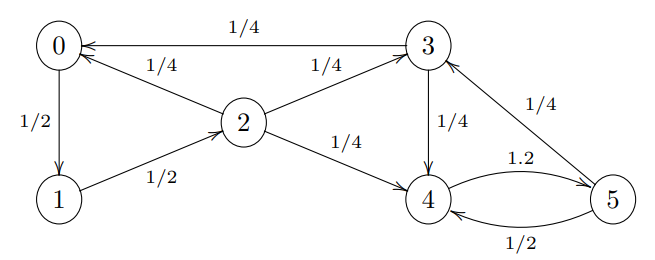
\includegraphics[width=.7\textwidth]{markov_ejer1_5}
\end{figure}

\textit{Se asume que cada estado tiene un ``self-loop'' con la probabilidad necesaria para que la suma de las probabilidades de salida sea $1$. Escribir un programa para contestar a las siguientes preguntas:}
\textit{
\begin{itemize}
\item[i)] Considerando $\lambda=(1,0,0,0,0,0)'$ (es decir, se empieza en el estado $0$), calcular $p(2)$, $p(10)$ y $p(100)$.
\item[ii)] Repetir los cálculos anteriores con $\lambda=(0,0,1,0,0,0)'$.
\item[iii)] Repetir los cálculos anteriores con $\lambda=(0,0,0,0,0,1)'$.
\item[(iv)] ¿Cómo cambian los tres vectores $p(2)$, $p(10)$ y $p(100)$? ¿Cómo cambia su dependencia de las condiciones iniciales? ¿Qué implica esto para $p(\infty)$?
\end{itemize}}

\textit{Solución}. En primer lugar escribimos la matriz de transición de esta cadena:

\[\Bigg
P = \begin{pmatrix}
  1/2 & 1/2 & 0 & 0 & 0 & 0\\
  0 & 1/2 & 1/2 & 0 & 0 & 0\\
  1/4 & 0 & 1/4 & 1/4 & 1/4 & 0\\
  1/4 & 0 & 0 & 1/2 & 1/4 & 0\\
  0 & 0 & 0 & 0 & 1/2 & 1/2\\
  0 & 0 & 0 & 1/4 & 1/2 & 1/4
\end{pmatrix}
\]

Escribimos un programa que, dada esta matriz $P$ y una distribución inicial $\lambda$, nos permita calcular $p(t)$ para cualquier $t$, empleando la fórmula demostrada en el apartado anterior.

\begin{minted}{python}
import numpy as np

# Transition matrix
P = np.array([[0.5, 0.5, 0, 0, 0, 0],
              [0, 0.5, 0.5, 0, 0, 0],
              [0.25, 0, 0.25, 0.25, 0.25, 0],
              [0.25, 0, 0, 0.5, 0.25, 0],
              [0, 0, 0, 0, 0.5, 0.5],
              [0, 0, 0, 0.25, 0.5, 0.25]])

# Initial distributions
l1 = np.array([1, 0, 0, 0, 0, 0])
l2 = np.array([0, 0, 1, 0, 0, 0])
l3 = np.array([0, 0, 0, 0, 0, 1])

# Desired future distributions
t1 = 2
t2 = 10
t3 = 100

# Print distributions p(t) up to 6 significant digits
np.set_printoptions(precision = 6, suppress = True)
for l in [l1, l2, l3]:
    print(f"Initial distribution: {l}")
    for t in [t1, t2, t3]:
        pt = l @ np.linalg.matrix_power(P, t)
        print(f"  p({t}) = {pt}")

\end{minted}

Si ejecutamos nuestro programa, obtenemos los siguientes resultados:

\begin{verbatim}
Initial distribution: [1 0 0 0 0 0]
  p(2) = [0.25 0.5  0.25 0.   0.   0.  ]
  p(10) = [0.13752  0.155167 0.113911 0.140522 0.279381 0.1735  ]
  p(100) = [0.111111 0.111111 0.074074 0.148148 0.333333 0.222222]
Initial distribution: [0 0 1 0 0 0]
  p(2) = [0.25   0.125  0.0625 0.1875 0.25   0.125 ]
  p(10) = [0.120958 0.127216 0.088414 0.145421 0.313589 0.204401]
  p(100) = [0.111111 0.111111 0.074074 0.148148 0.333333 0.222222]
Initial distribution: [0 0 0 0 0 1]
  p(2) = [0.0625 0.     0.     0.1875 0.4375 0.3125]
  p(10) = [0.102201 0.096315 0.060696 0.150693 0.351478 0.238618]
  p(100) = [0.111111 0.111111 0.074074 0.148148 0.333333 0.222222]
\end{verbatim}

Como vemos, el vector $p(2)$ es distinto en los tres casos, el vector $p(10)$ es tan solo ligeramente distinto, y $p(100)$ es ya igual para todas las condiciones iniciales probadas. Esto es, hay una convergencia al estado $p(100)$ en los tres casos, aunque dependiendo de la condición inicial esta convergencia es más lenta o más rápida. Esto nos hace pensar que el estado $p(100)$ es el ``estado final'' de la cadena, que podemos denotar como $p(\infty) = \lim_{t\to\infty} p(t)$. De hecho, se comprueba analíticamente que para estos tres estados iniciales se verifica
\[
p(101)'=p(100)'P = p(100)',
\]

luego por la característica de falta de memoria de las cadenas de Markov, concluimos que $p(100 + \tau)=p(100)$ $\forall \tau > 0$. Por tanto, podemos afirmar que efectivamente $p(\infty)=p(100)$. Más aún, atendiendo a la fórmula del apartado anterior, si existe el límite se tendría
\[
p(\infty) = \lambda' \lim_{t\to\infty} P^t = \lambda' P^\infty,
\]

y si $P$ fuera diagonalizable (sobre los complejos), existirían una matriz $D$ diagonal y una matriz $V$ invertible tales que
\[
P^t = VD^tV^{-1} \quad \forall t.
\]

Si, por ejemplo, todas las entradas diagonales de la matriz $D$ o bien fueran $1$ o bien tuvieran módulo menor que 1, podríamos calcular fácilmente $\lim_{t\to\infty} D^t$ (nos quedarían solamente 0s y 1s en la diagonal), y por tanto calcular $P^\infty$. Resulta que en este caso podemos hacer justamente eso:

\begin{minted}{python}
# Compute limiting transition matrix
l, v = np.linalg.eig(P)
l[np.abs(l) < 1] = 0
d = np.diag(l)
p_inf = np.real_if_close(v @ d @ np.linalg.inv(v))
\end{minted}

Comprobamos que como salida obtenemos la siguiente matriz:
\[
P^{\infty} = \begin{pmatrix}
  0.111111 & 0.111111 & 0.074074 & 0.148148 & 0.333333 & 0.222222\\
  0.111111 & 0.111111 & 0.074074 & 0.148148 & 0.333333 & 0.222222\\
  0.111111 & 0.111111 & 0.074074 & 0.148148 & 0.333333 & 0.222222\\
  0.111111 & 0.111111 & 0.074074 & 0.148148 & 0.333333 & 0.222222\\
  0.111111 & 0.111111 & 0.074074 & 0.148148 & 0.333333 & 0.222222\\
  0.111111 & 0.111111 & 0.074074 & 0.148148 & 0.333333 & 0.222222
\end{pmatrix},
\]

que vemos que no es más que la matriz cuyas filas son $p(\infty)'$. A la vista de esta matriz podemos concluir que la cadena no solo convergerá a $p(\infty)$ partiendo de los estados iniciales que hemos comprobado, sino que tenderá a este estado sea quien sea la condición inicial, incluso aunque las probabilidades iniciales se repartan y no se concentren en un único estado.

\end{document}
